\chapter{Tone Output using an Arduino}

Overview

This lab is an introduction to generating simple tones on an Arduino. NOTE: This will work only for Arduino 0018 and beyond. For previous versions, use Brett Hagman's Tone library

For this lab you'll need:

Solderless breadboard


\begin{figure}[!htb]
 \centering
 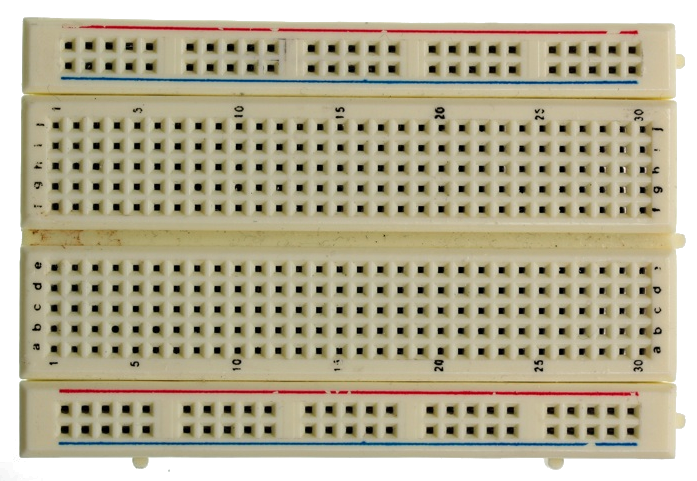
\includegraphics[scale=0.3]{img/toneout/breadboard.png}
 \caption{breadboard}
 \label{breadboard}
\end{figure}


22-AWG hookup wire


\begin{figure}[!htb]
 \centering
 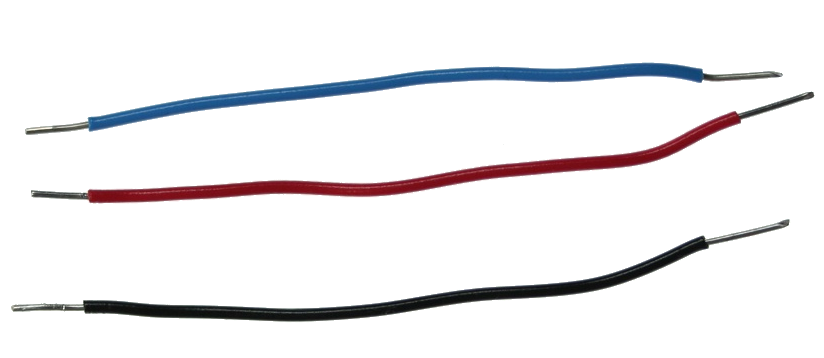
\includegraphics[scale=0.3]{img/toneout/hookup_wire.png}
 \caption{hookup wire}
 \label{hookup wire}
\end{figure}

Arduino Microcontroller module


\begin{figure}[!htb]
 \centering
 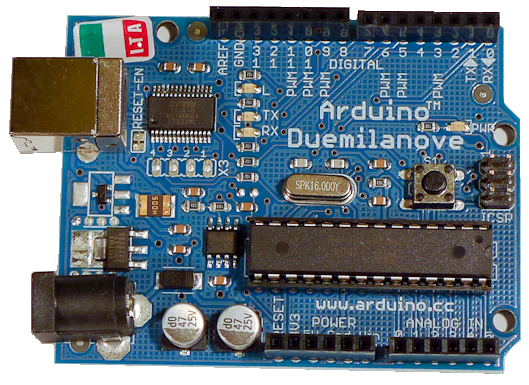
\includegraphics[scale=0.3]{img/toneout/arduino.png}
 \caption{arduino}
 \label{arduino}
\end{figure}


1Kohm resistors


\begin{figure}[!htb]
 \centering
 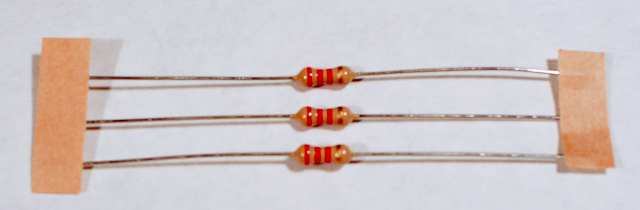
\includegraphics[scale=0.3]{img/toneout/resistors.jpg}
 \caption{resistors}
 \label{resistors}
\end{figure}

photocell (or a different form of variable resistor)
 

\begin{figure}[!htb]
 \centering
 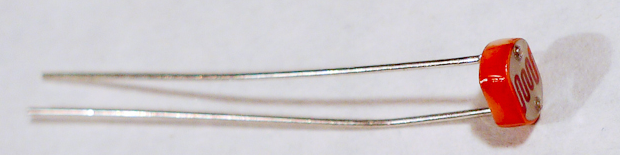
\includegraphics[scale=0.3]{img/toneout/photocell.png}
 \caption{photocell}
 \label{photocell}
\end{figure}

8-ohm speaker


\begin{figure}[!htb]
 \centering
 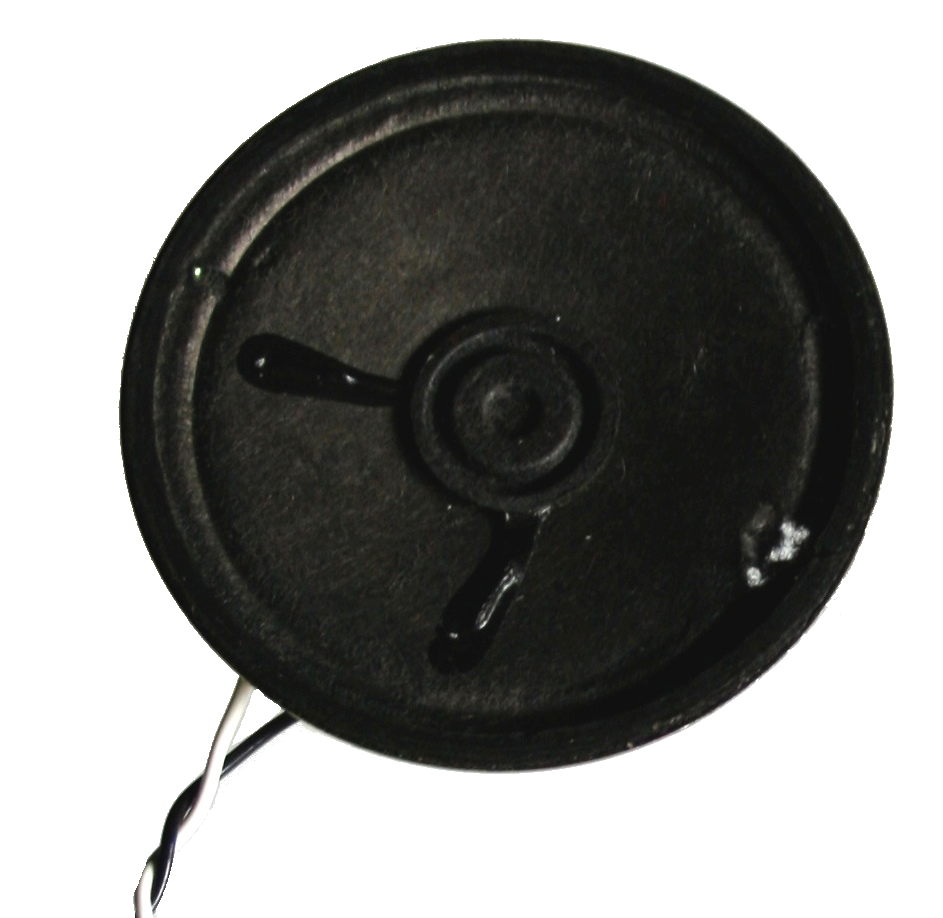
\includegraphics[scale=0.15]{img/toneout/speaker.png}
 \caption{speaker}
 \label{speaker}
\end{figure}


\section{Why not use AnalogOut()?}

When you use analogOut() to create pulsewidth modulation (PWM) on an output pin, you can change the on-off ratio of the output (also known as the duty cycle) but not the frequency. If you have a speaker connected to an output pin running analogOut(), you'll get a changing loudness, but a constant tone. To change the tone, you need to change the frequency. The tone() command does this for you.

\section{Prepare the breadboard}

Connect power and ground on the breadboard to power and ground from the microcontroller. On the Arduino module, use the 5V and any of the ground connections:

\begin{figure}[!htb]
 \centering
 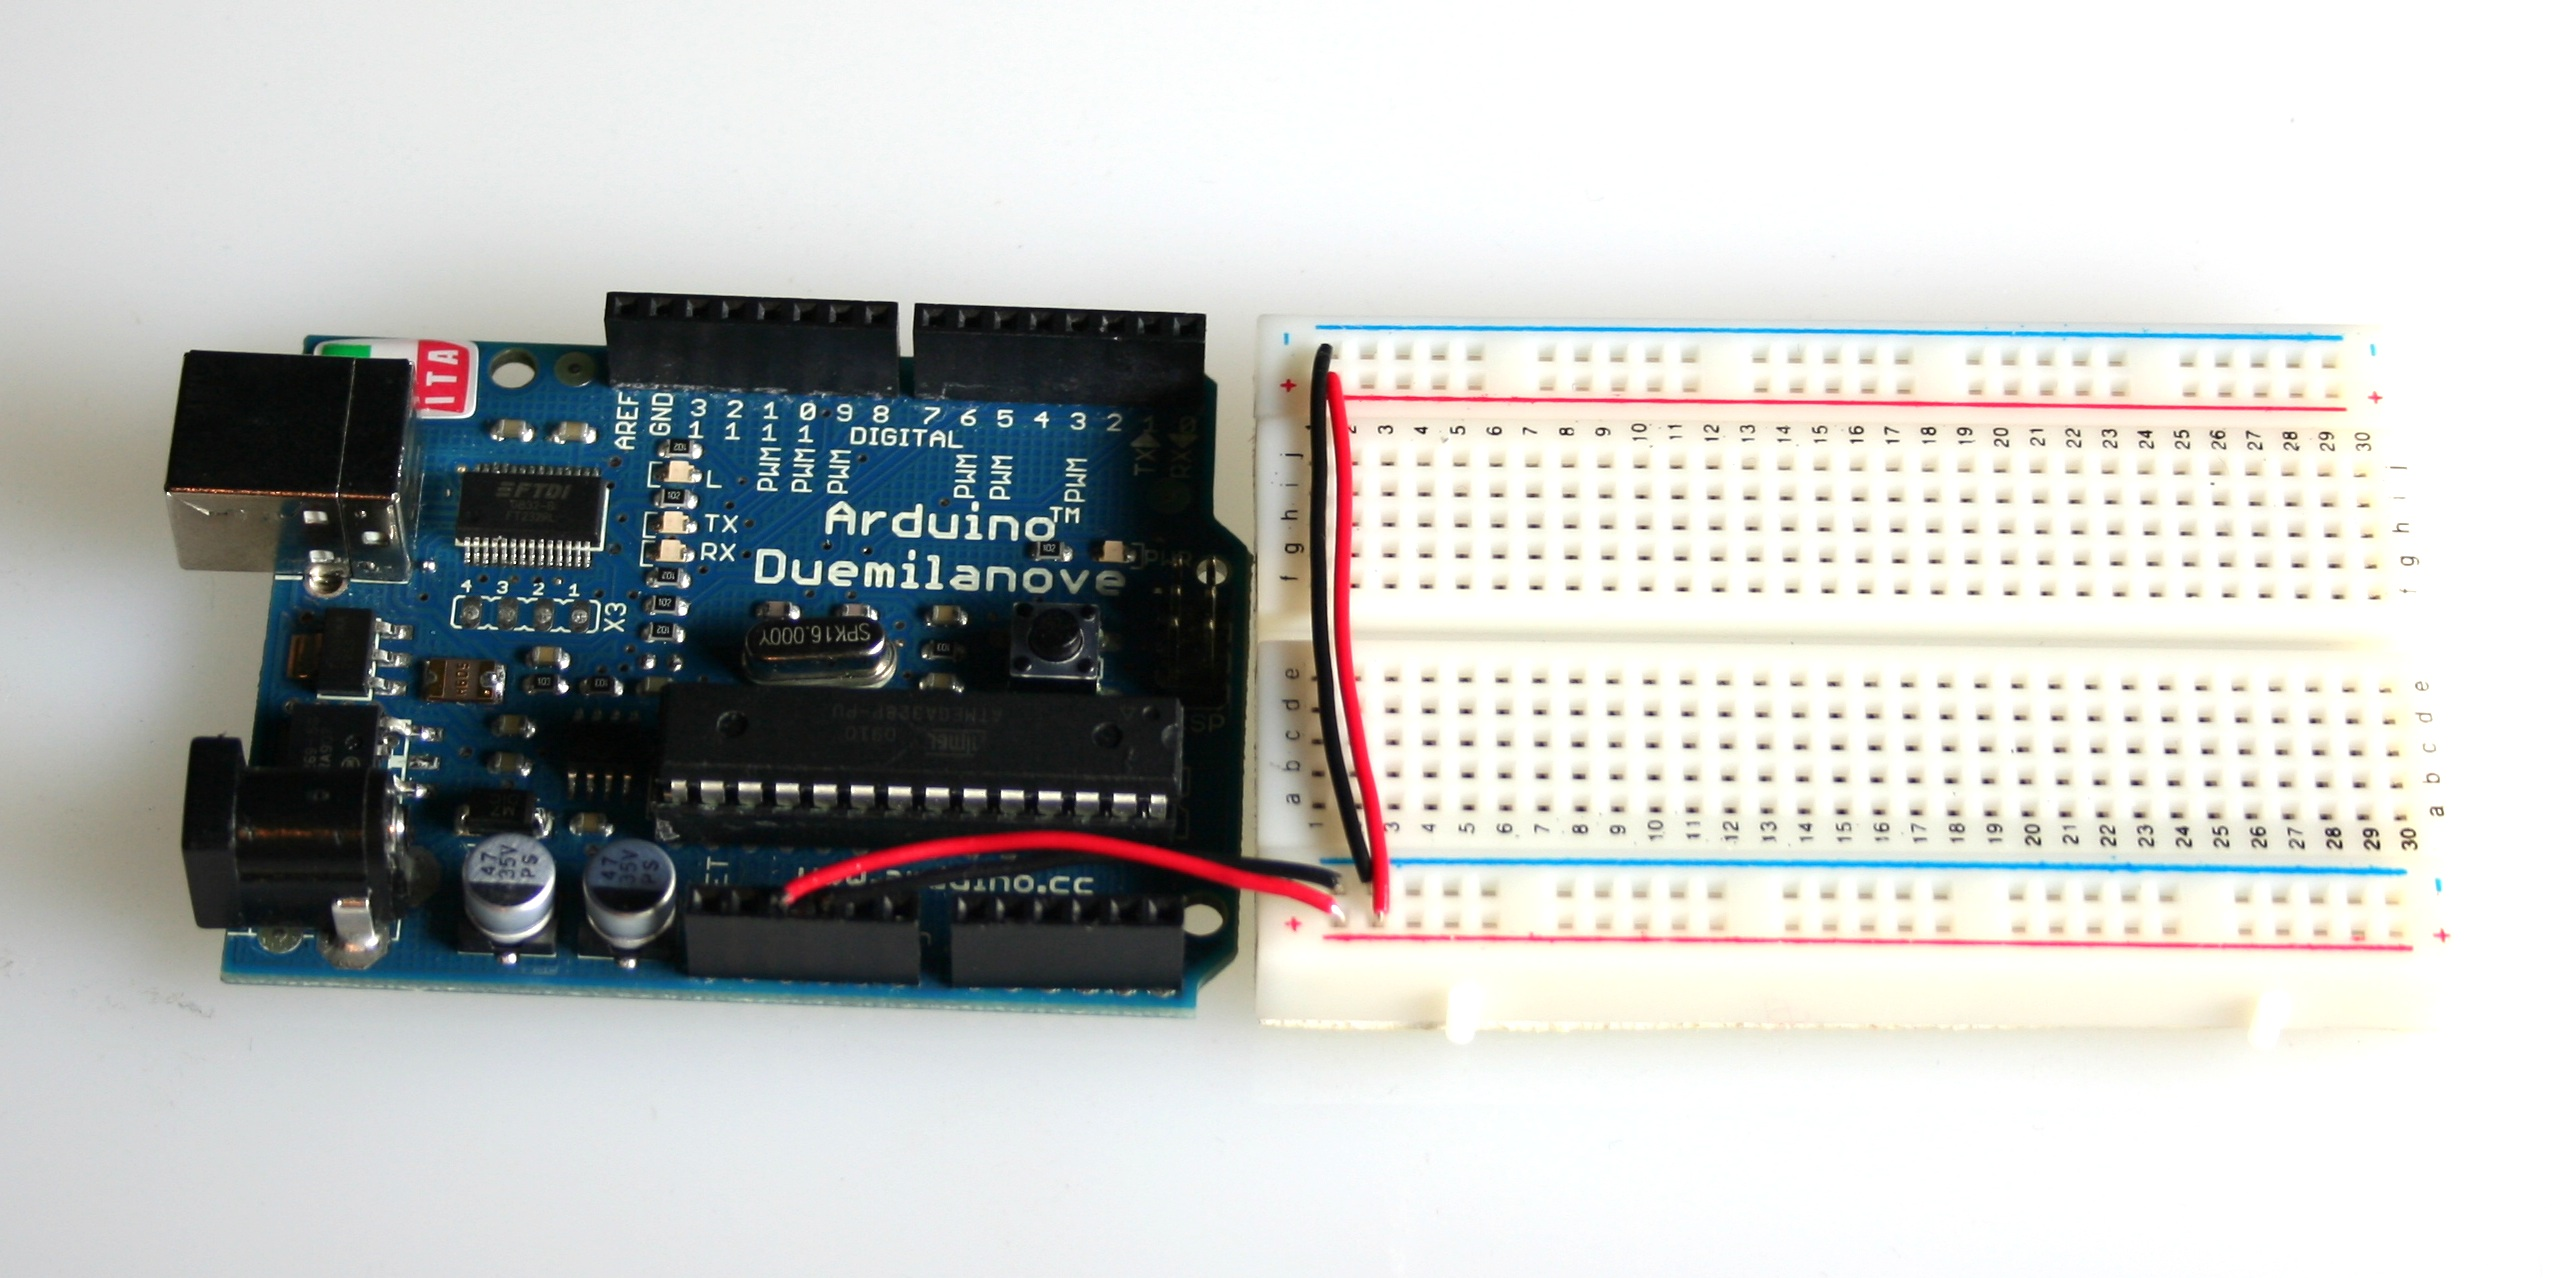
\includegraphics[scale=0.1]{img/toneout/arduino_breadboard_power.jpg}
 \caption{arduino breadboard power}
 \label{arduino breadboard power}
\end{figure}

\begin{figure}[!htb]
 \centering
 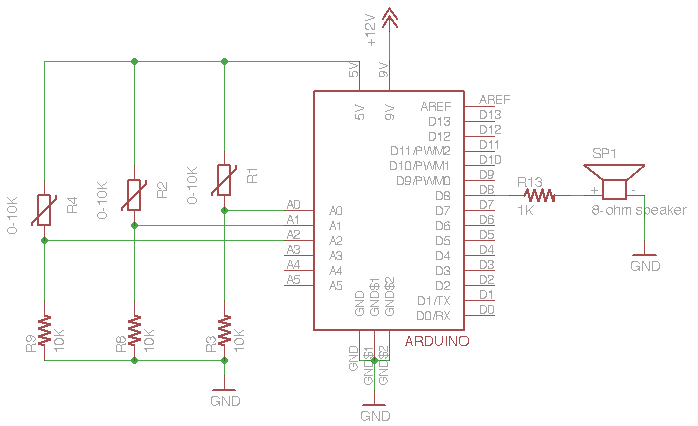
\includegraphics[scale=0.3]{img/toneout/toneKeyboard_schem.png}
 \caption{toneKeyboard schem}
 \label{toneKeyboard schem}
\end{figure}


\section{Connect the sensors and the speaker}

Connect two photoresistors to analog pin 0 in a voltage divider circuit as shown below. The 8-ohm speaker connects to pin 8 of the Arduino. You can use any digital I/O pin if you don't like 8. The other end of the speaker connects to ground.


\begin{figure}[!htb]
 \centering
 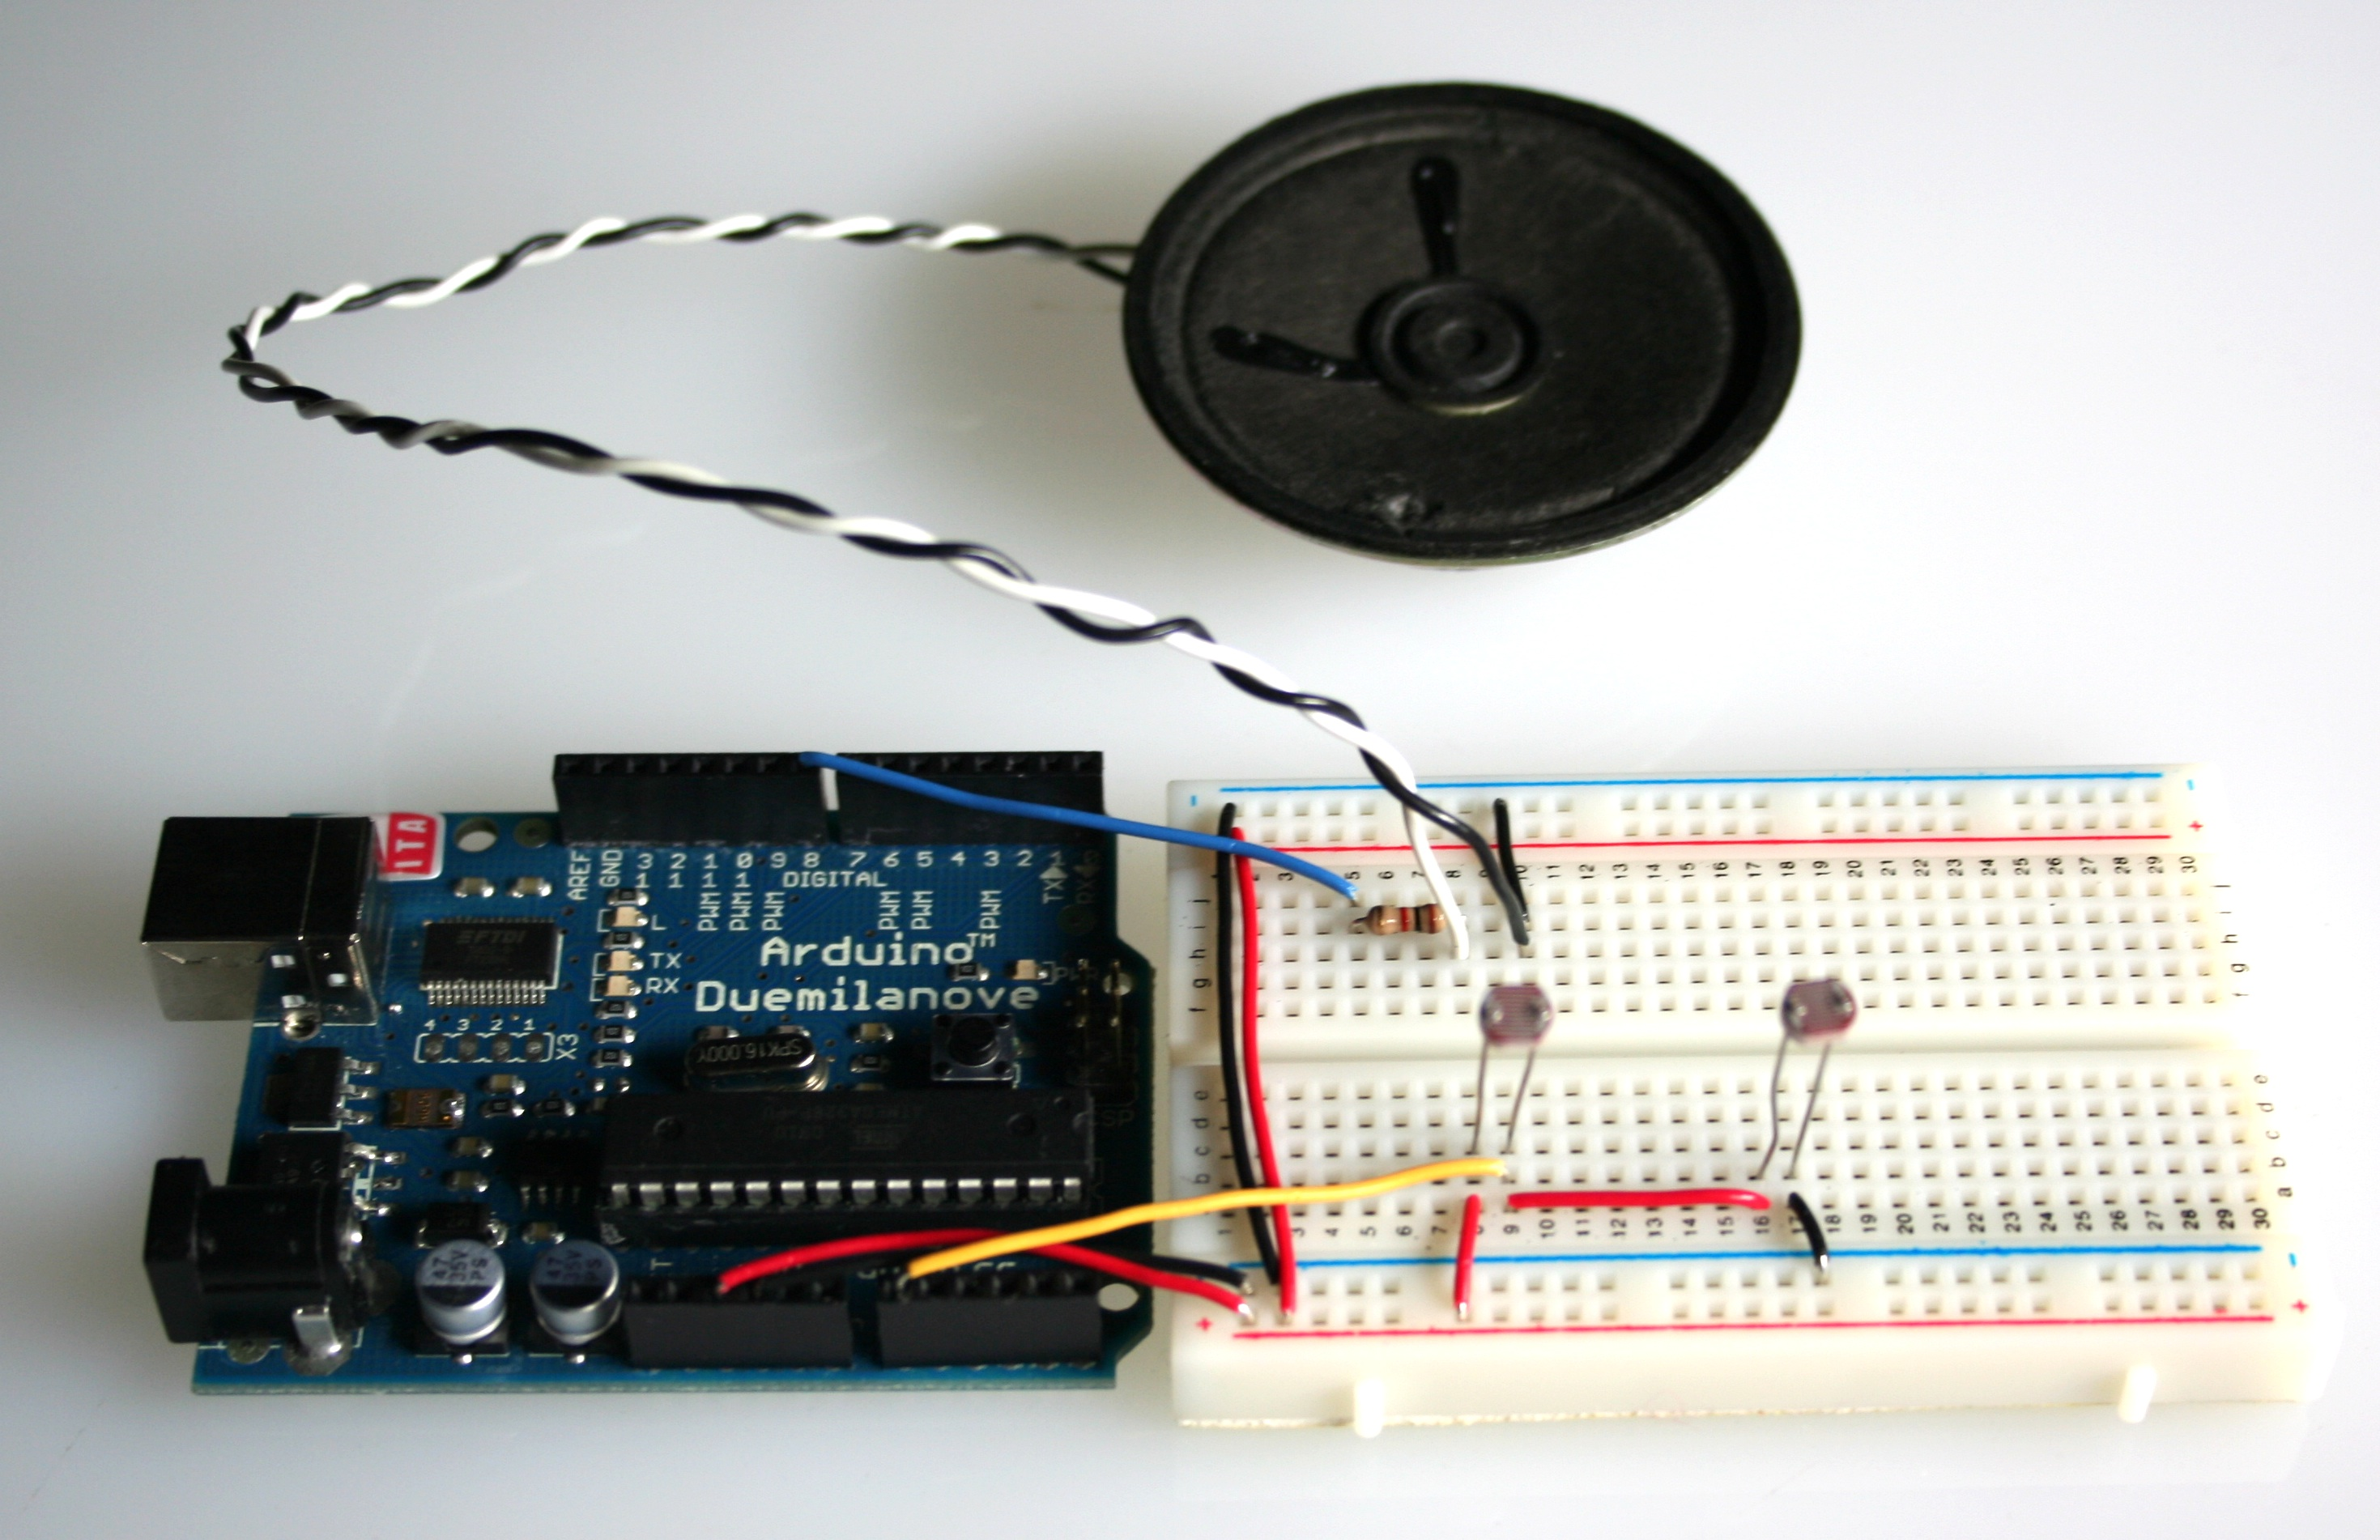
\includegraphics[scale=0.1]{img/toneout/photocell_bb.jpg}
 \caption{photocell bb}
 \label{photocell bb}
\end{figure}


NOTE: this sensor circuit is not the normal way of connecting an analog input. There is no fixed resistor. The two photocells act as a voltage divider together, ao you can change the value of the analog in by covering either one. if you are using variable resistors that can both go to 0 ohms, you should connect a fixed resistor in series from the junction of the two resistors to the input, to avoid a short.

\section{Check the sensor input range}

Once you've got the circuit connected, check the range of the analog input with the following code:
 void setup() {
   Serial.begin(9600);
 }

 void loop() {
   int sensorValue = analogRead(0);
   Serial.println(sensorValue, DEC);
 }
Note the range that the sensors give you by alternately covering them up and giving them full light, with the serial monitor window all the time. You'll need the maximum and minimum sensor values for the next sketch.

\section{Play Tones}

The sketch below takes input from the photocells and uses it to generate tones on the speaker. Upload it to your Arduino, and see the effect.

\begin{lstlisting}[language=C]
 /*
   Theremin
  
  Plays tones based on a sensor reading
  
  circuit:
  * photoresistor from +5V to analog in 0
  * photoresistor from analog pin 0 to ground
  * 8-ohm speaker on digital pin 8
  
  created 10 Sep 2009
  modified 8 Feb 2009
  by Tom Igoe 
  */


 void setup() {

 }

 void loop() {
   // get a sensor reading:
   int sensorReading = analogRead(0);
   // map the results from the sensor reading's range
   // to the desired pitch range:
   int pitch = map(sensorReading, 200, 900, 100, 1000);
   // change the pitch, play for 10 ms:
   tone(8, pitch, 10);
 }
\end{lstlisting}

\section{A more complex example}

The pitches.h file includes constants that give you the pitches for a standard western scale. Here's an example that uses them to play a simple melody:
\begin{lstlisting}[language=C]
 /*
   Melody
  
  Plays a melody 
  
  circuit:
  * 8-ohm speaker on digital pin 8
  
  created 21 Jan 2010
  by Tom Igoe 
  */
 #include "pitches.h"

 // notes in the melody:
 int melody[] = {
   NOTE_C4, NOTE_G3,NOTE_G3, NOTE_A3, NOTE_G3,0, NOTE_B3, NOTE_C4};

 // note durations: 4 = quarter note, 8 = eighth note, etc.:
 int noteDurations[] = {
   4, 8, 8, 4,4,4,4,4 };

 void setup() {
   // iterate over the notes of the melody:
   for (int thisNote = 0; thisNote < 8; thisNote++) {

     // to calculate the note duration, take one second 
     // divided by the note type.
     //e.g. quarter note = 1000 / 4, eighth note = 1000/8, etc.
     int noteDuration = 1000/noteDurations[thisNote];
     tone(8, melody[thisNote],noteDuration);

     // to distinguish the notes, set a minimum time between them.
     // the note's duration + 30% seems to work well:
     int pauseBetweenNotes = noteDuration * 1.30;
     delay(pauseBetweenNotes);
   }
 }

 void loop() {
   // no need to repeat the melody.
 }
\end{lstlisting}
Here's an example of how to use the note constants to make a simple keyboard:
The circuit:


This circuit uses the more traditional voltage divider circuit.
\begin{lstlisting}[language=C]
 /*
   keyboard
  
  Plays a pitch that changes based on a changing analog input
  
  circuit:
  * 3 force-sensing resistors from +5V to analog in 0 through 5
  * 3 10K resistors from analog in 0 through 5 to ground
  * 8-ohm speaker on digital pin 8
  
  created 21 Jan 2010
  by Tom Igoe 
  
  */

 #include "pitches.h"

 const int threshold = 10;    // minimum reading of the sensors that generates a note

 // notes to play, corresponding to the 3 sensors:
 int notes[] = {
   NOTE_A4, NOTE_B4,NOTE_C3 };

 void setup() {

 }

 void loop() {
   for (int thisSensor = 0; thisSensor < 3; thisSensor++) {
     // get a sensor reading:
     int sensorReading = analogRead(thisSensor);

     // if the sensor is pressed hard enough:
     if (sensorReading > threshold) {
       // play the note corresponding to this sensor:
       tone(8, notes[thisSensor], 20);
     } 
   }
   Serial.println();
 }
\end{lstlisting}

\section{Make an Instrument}

This is a suggestion for the Media Controller assignment. You can do any project you wish as long as it demonstrates your mastery of the lab exercises and good physical interaction. This is just one suggestion.

Now that you've got the basics, make a musical instrument. Consider a few things in designing yor instrument:

\begin{itemize}
\item Do you want to play discrete notes (like a piano), or sliding pitches (like a theremin)? How do you program to achieve these effects?
\item Do you want to control the tempo and duration of a note?
\item Do you want the same physical action to set both the pitch and the velocity (volume) of a note?
\item Do you want to be able to play more than one note at a time (e.g. chords)?
\end{itemize}

All of these questions, and many more, will affect what sensors you use, how you read them, and how you design both the physical interface and the software.


\begin{figure}[!htb]
 \centering
 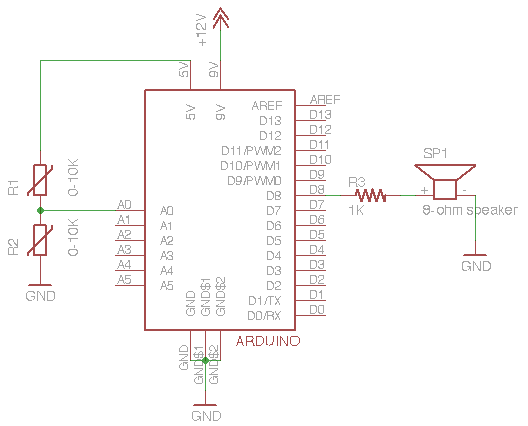
\includegraphics[scale=1]{img/toneout/photocell_schem.png}
 \caption{photocell schem}
 \label{photocell schem}
\end{figure}




\begin{figure}[!htb]
 \centering
 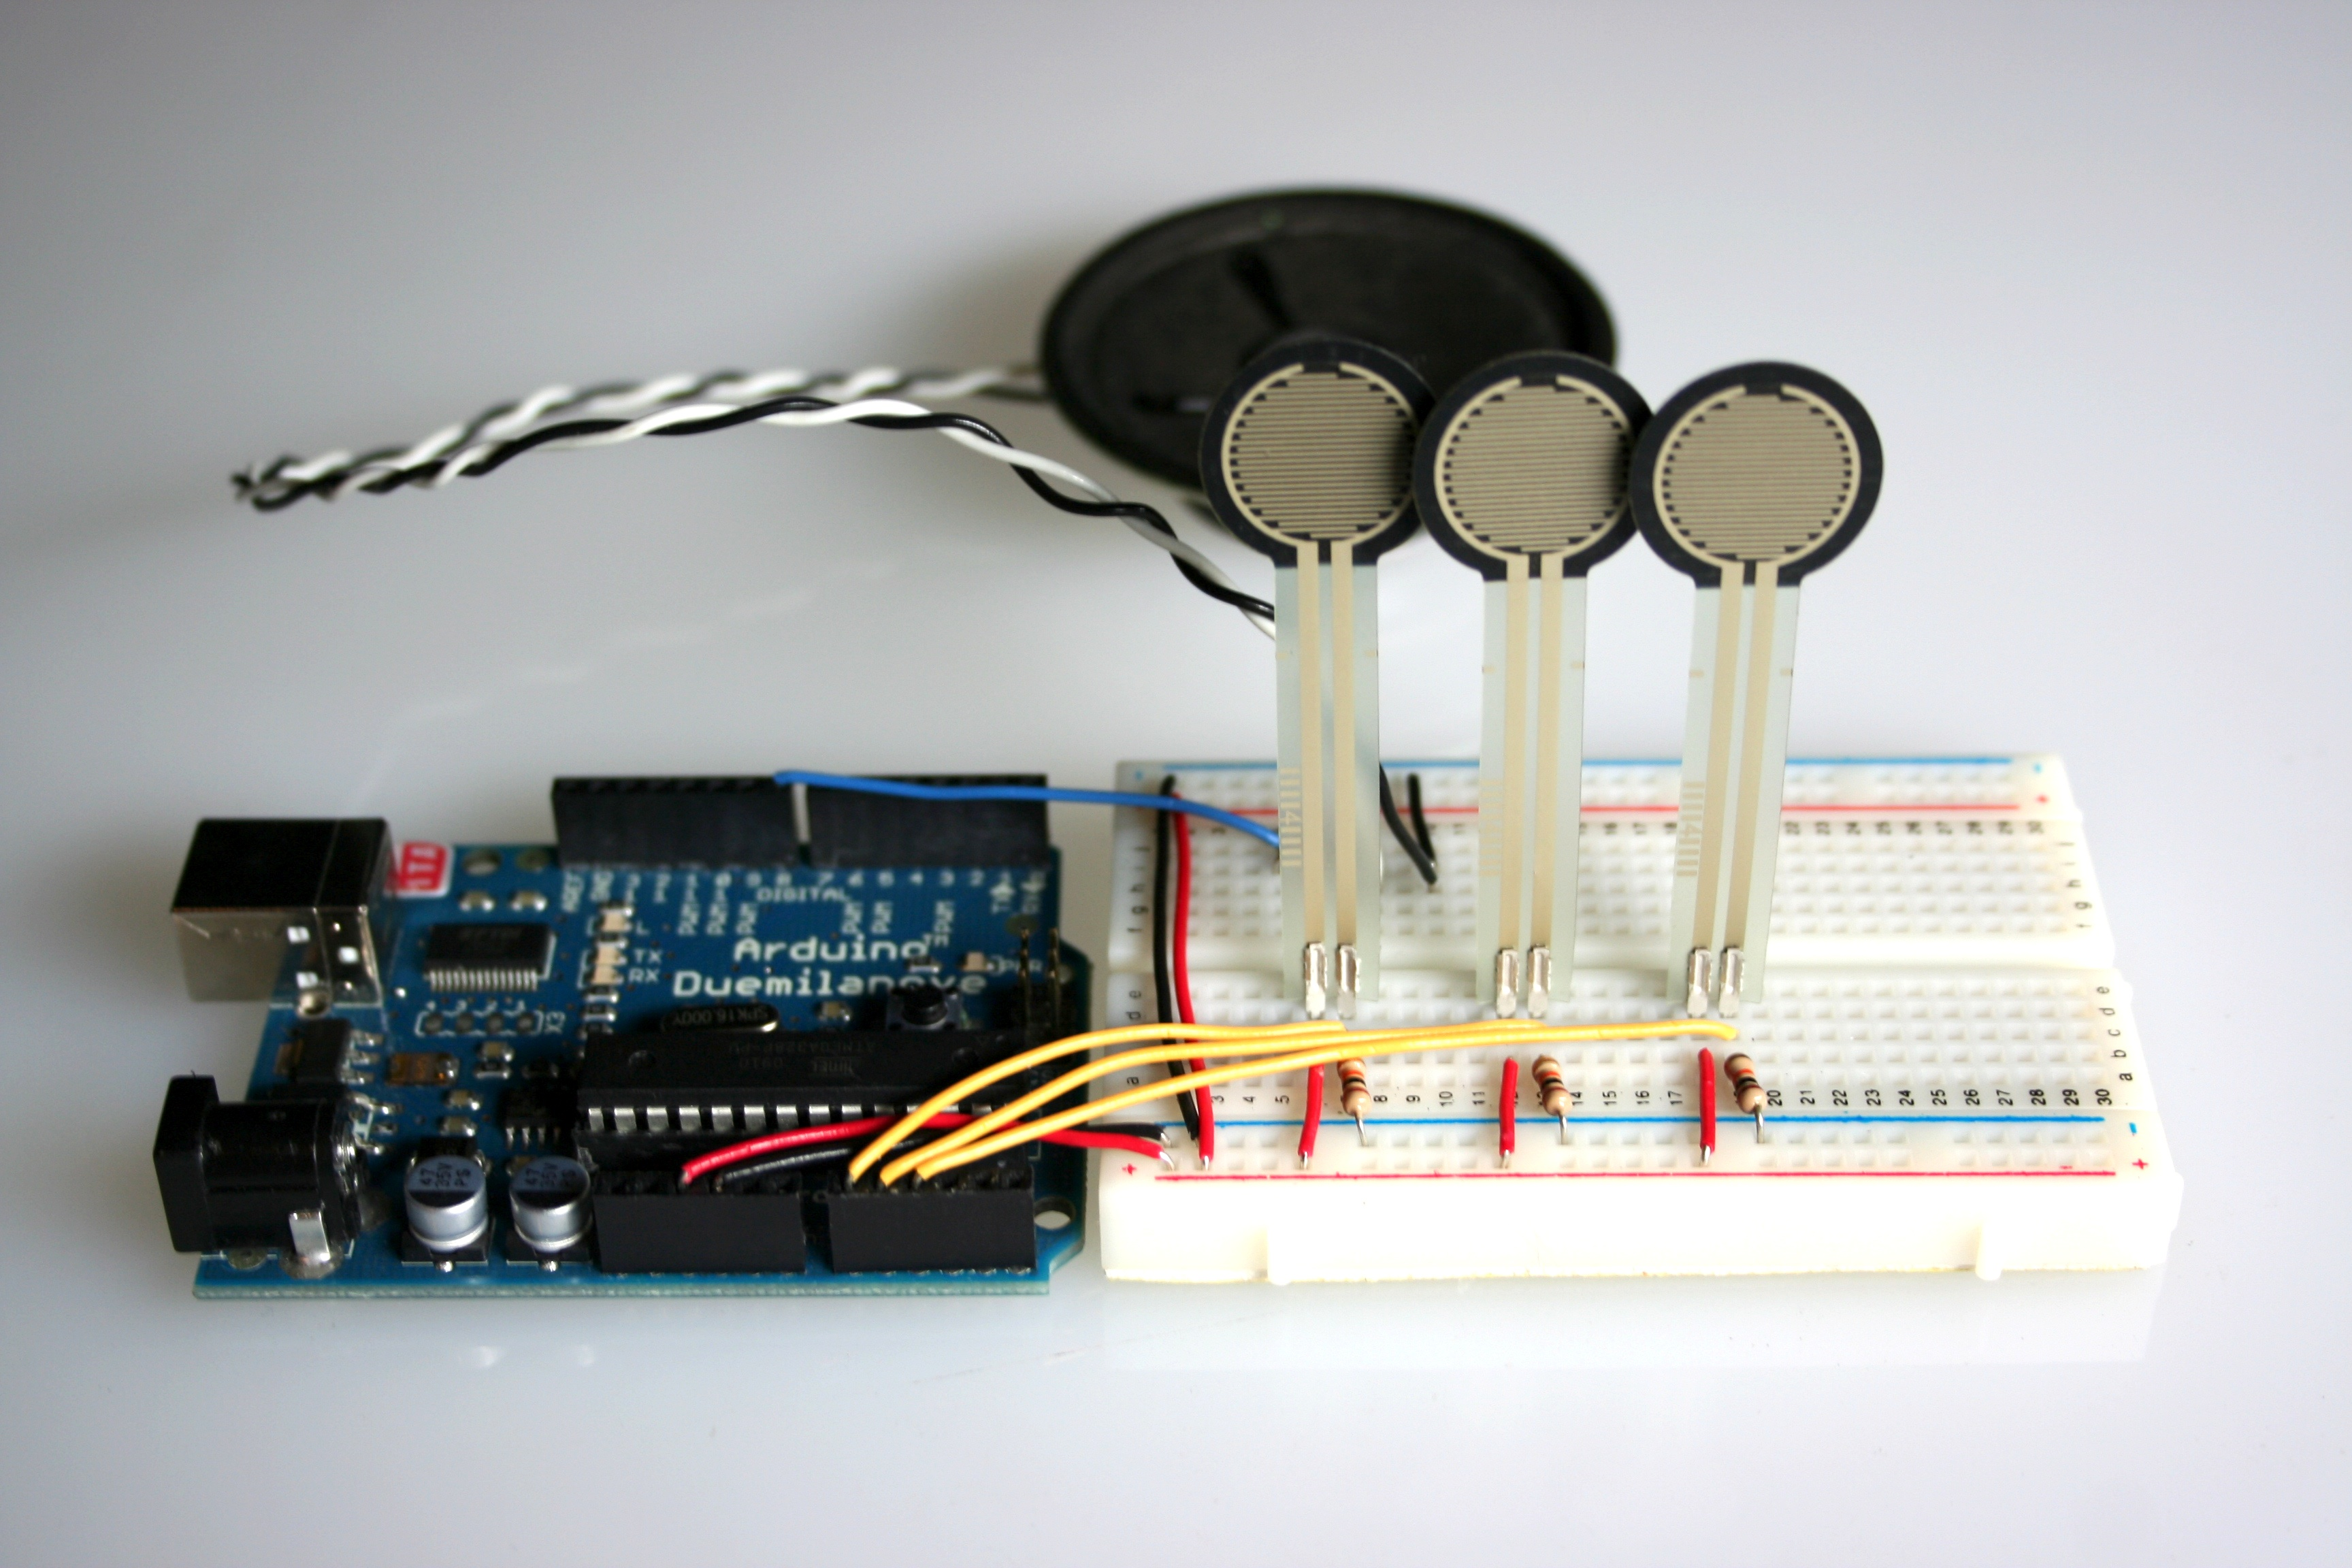
\includegraphics[scale=0.1]{img/toneout/toneKeyboard_bb.jpg}
 \caption{toneKeyboard bb}
 \label{toneKeyboard bb}
\end{figure}



